\documentclass[border=10pt]{standalone}
\usepackage[svgnames]{xcolor}
\usepackage{amsmath}
\usepackage{pgfplots}
\pgfplotsset{compat=newest}
\usepackage[sfdefault]{FiraSans}
\usepackage{FiraMono}
\renewcommand*\familydefault{\sfdefault}
\begin{document}
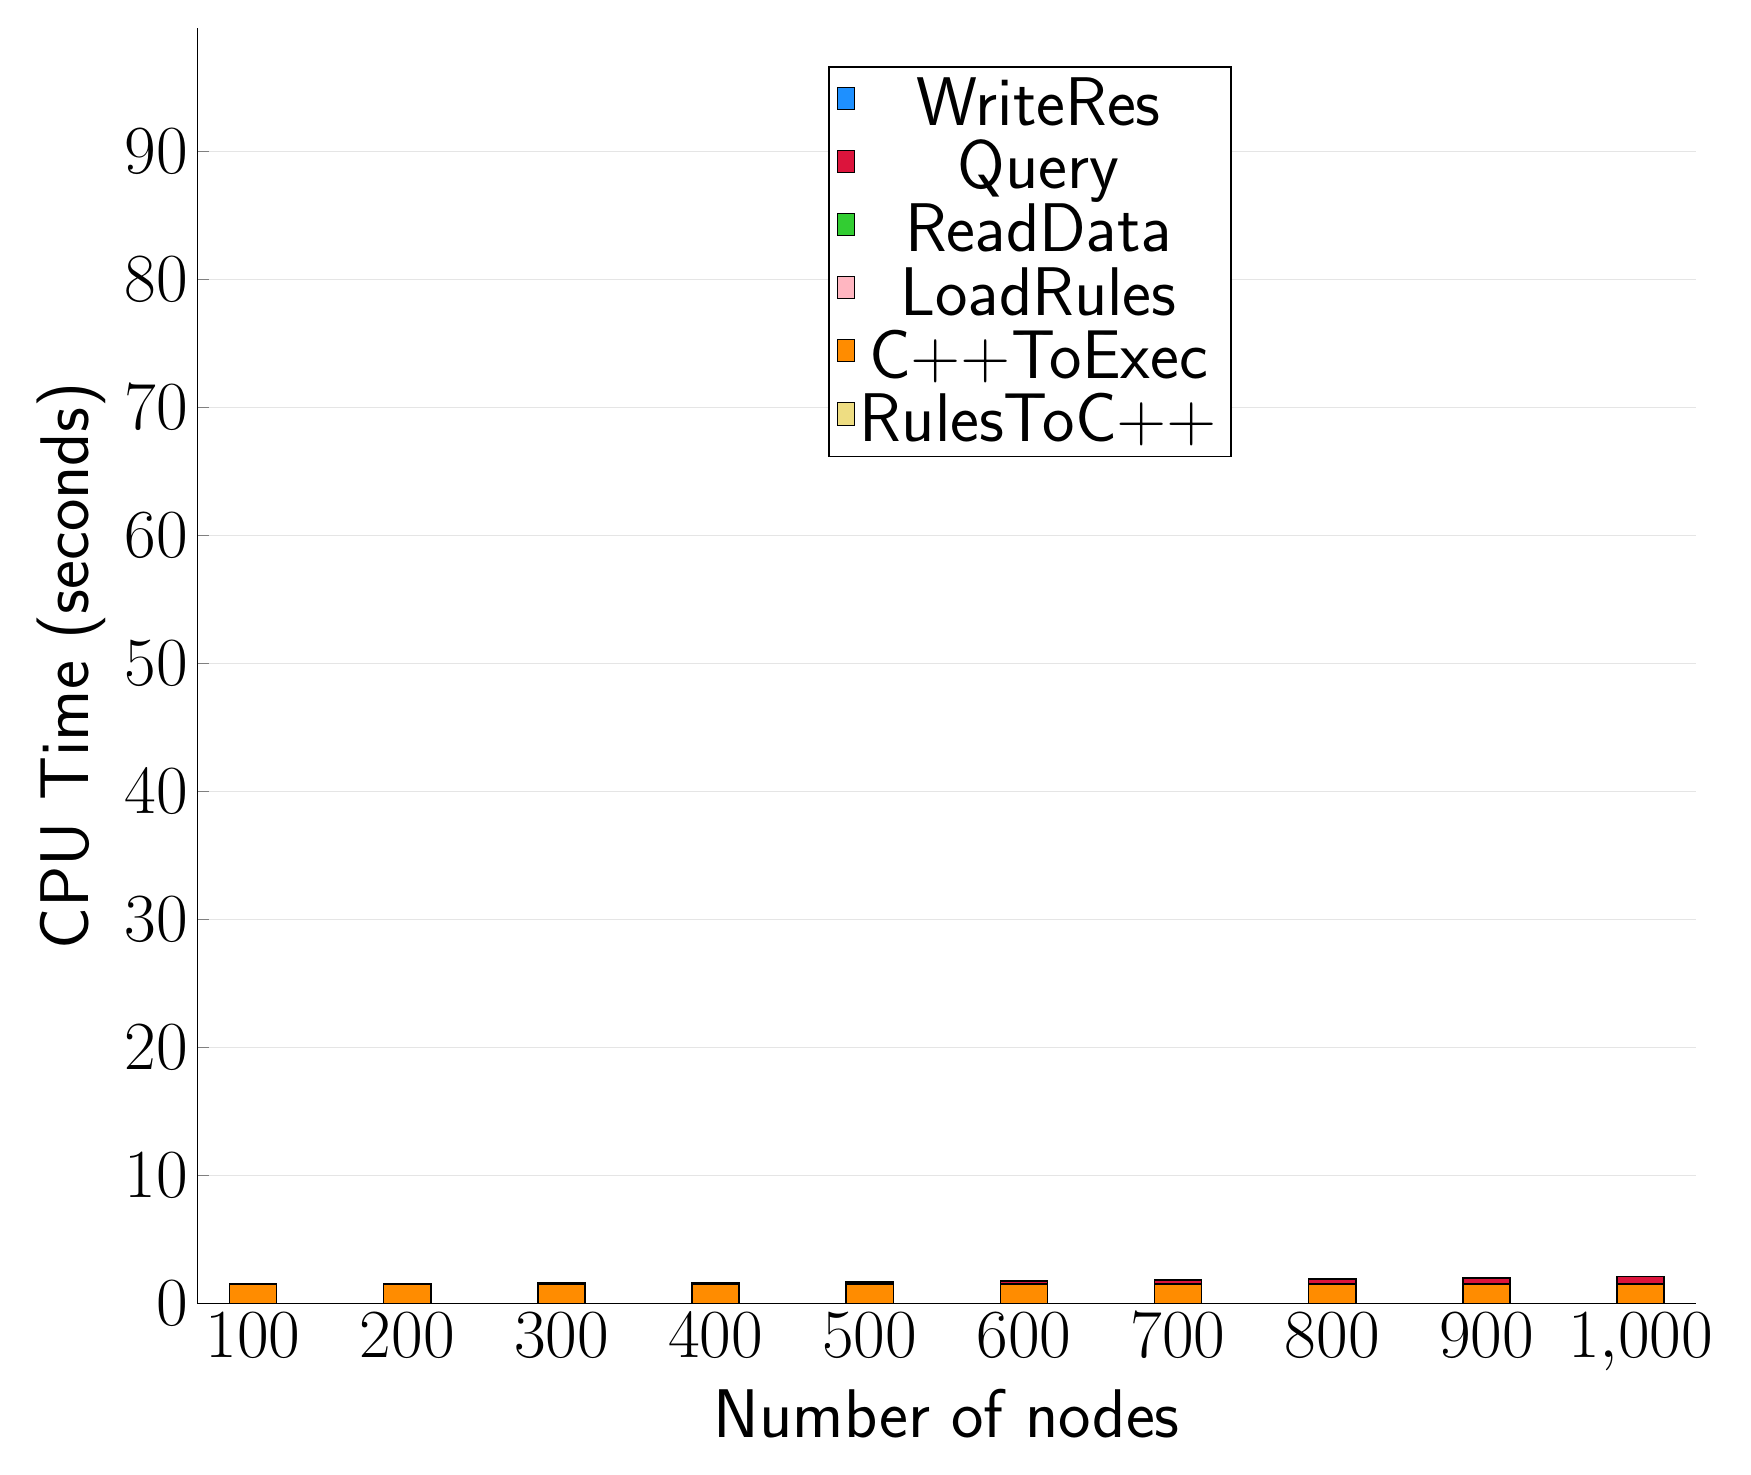
\begin{tikzpicture}
\begin{axis}[
   ybar stacked,
   width=1.7\textwidth,
   bar width=0.6cm,
   ymajorgrids, tick align=inside,
   major grid style={draw=gray!20},
   xtick=data,
   ymin=0, ymax=99.5987,
   axis x line*=bottom,
   axis y line*=left,
   enlarge x limits=0.04,
   legend style={
       at={(0.69, 0.97)},
       anchor=north east,
       legend columns=1,
       font=\Huge,
   },
   ylabel={CPU Time (seconds)},
   xlabel={Number of nodes},
   label style={font=\Huge},
   tick label style={font=\Huge},
]
\addlegendimage{fill=DodgerBlue, draw=black, line width=0.2pt}
\addlegendentry{WriteRes}
\addlegendimage{fill=Crimson, draw=black, line width=0.2pt}
\addlegendentry{Query}
\addlegendimage{fill=LimeGreen, draw=black, line width=0.2pt}
\addlegendentry{ReadData}
\addlegendimage{fill=LightPink, draw=black, line width=0.2pt}
\addlegendentry{LoadRules}
\addlegendimage{fill=DarkOrange, draw=black, line width=0.2pt}
\addlegendentry{C++ToExec}
\addlegendimage{fill=LightGoldenrod, draw=black, line width=0.2pt}
\addlegendentry{RulesToC++}
\addplot +[fill=LightGoldenrod, draw=black, line width=0.55pt] coordinates {
(100, 0.0)
(200, 0.0020000000000000005)
(300, 0.008000000000000002)
(400, 0.008000000000000002)
(500, 0.010000000000000002)
(600, 0.010000000000000002)
(700, 0.010000000000000002)
(800, 0.006000000000000001)
(900, 0.008000000000000002)
(1000, 0.008000000000000002)
};
\addplot +[fill=DarkOrange, draw=black, line width=0.55pt] coordinates {
(100, 1.514)
(200, 1.53)
(300, 1.526)
(400, 1.534)
(500, 1.52)
(600, 1.528)
(700, 1.5260000000000002)
(800, 1.528)
(900, 1.53)
(1000, 1.508)
};
\addplot +[fill=LightPink, draw=black, line width=0.55pt] coordinates {
(100, 0.0001414)
(200, 0.0001482)
(300, 0.0001588)
(400, 0.000149)
(500, 0.0001304)
(600, 0.0001504)
(700, 0.0001472)
(800, 0.0001596)
(900, 0.00014419999999999998)
(1000, 0.00015120000000000002)
};
\addplot +[fill=LimeGreen, draw=black, line width=0.55pt] coordinates {
(100, 0.0008642000000000001)
(200, 0.0012182)
(300, 0.0016382)
(400, 0.0020128000000000004)
(500, 0.0021688)
(600, 0.0027218000000000003)
(700, 0.0031551999999999995)
(800, 0.0034102)
(900, 0.0034844)
(1000, 0.0037635999999999998)
};
\addplot +[fill=Crimson, draw=black, line width=0.55pt] coordinates {
(100, 0.009730800000000001)
(200, 0.0354004)
(300, 0.067496)
(400, 0.10575540000000001)
(500, 0.1536676)
(600, 0.21744819999999998)
(700, 0.29225819999999997)
(800, 0.3795674)
(900, 0.4783284)
(1000, 0.5979715999999999)
};
\addplot +[fill=DodgerBlue, draw=black, line width=0.55pt] coordinates {
(100, 0.00027100000000000003)
(200, 0.00028460000000000003)
(300, 0.0002474)
(400, 0.0002582)
(500, 0.00026039999999999993)
(600, 0.0002634)
(700, 0.00028599999999999996)
(800, 0.0003316)
(900, 0.0003118)
(1000, 0.00033099999999999997)
};
\end{axis}
\end{tikzpicture}

\end{document}
